\chapter{Implementation  Process}

\section{Design Overview}

The design of Medora was guided by a strong emphasis on usability, comfort, and accessibility, ensuring that elderly users and individuals with limited technical literacy could interact with the system without difficulty. Medora was not intended to be a mobile robot; rather, it was conceptualized as a stationary assistive system that blends into a domestic environment while offering reliable healthcare support. The design journey progressed through three key stages: establishing a user-centered philosophy, conceptualizing a 3D design, and finally developing a functional working prototype.

\subsection{User-Centered Design}

A user-centered design approach was adopted to ensure Medora was welcoming and approachable for elderly users. The form factor was inspired by familiar household objects, particularly a table lamp, to evoke comfort and reduce any feelings of anxiety commonly associated with medical or robotic devices. The stationary structure allows the robot to be placed conveniently on bedside tables, kitchen counters, or desks without occupying much space.  

Interaction points were deliberately kept simple, intuitive, and highly accessible. Large tactile buttons, a bright high-contrast touchscreen, and voice interaction capabilities were integrated to accommodate users with reduced dexterity or vision impairments. Every design choice—from rounded edges to non-intimidating aesthetics—was made with inclusivity and ease of use in mind. This ensured that Medora not only performed its medical functions but also provided a sense of reassurance and trust to its primary users.

\subsection{3D Design for the Medora}

The 3D design of Medora was carefully crafted to translate the user-centered philosophy into a practical form. Its compact, ergonomic shape makes it suitable for placement in domestic environments, while smooth curves and a minimalistic aesthetic make it visually appealing.  

The proposed design highlights user interaction through a combination of physical and digital elements. The touchscreen interface displays essential information such as medication schedules, reminders, and health updates, while voice commands provide an alternative hands-free mode of interaction. The medicine dispensing area was modeled with logical compartmentalization, ensuring clear labeling, visible indicators, and safe, easy access. Additional safety features such as child-proof mechanisms can be incorporated without affecting usability.  

This stage of the design provided a virtual representation of Medora’s intended functionality, ensuring that the structure was both technically feasible and user-friendly before physical prototyping.  

\begin{figure}[H]
    \centering
    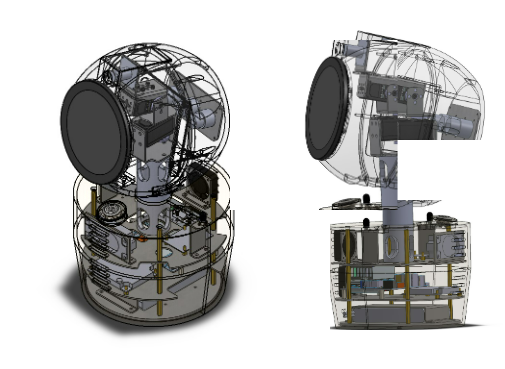
\includegraphics[width=0.5\textwidth]{pics/thesis/3D.drawio.png}
    \caption{Proposed 3D design of Medora}
    \label{fig:3d-design-medora}
\end{figure}

\subsection{Developed Prototype of Medora}

Following the conceptual design, Medora was developed into a functional working prototype through 3D printing and assembly. The final prototype retained the user-friendly, lamp-inspired form factor, providing a non-threatening appearance while integrating all key modules.  

From the \textbf{front view}, the main user interaction points are visible:  
\begin{itemize}
    \item A 5-inch touchscreen display serves as the primary interface for navigating medication reminders, health updates, and system alerts.  
    \item A webcam mounted above the screen enables facial recognition for personalization and user authentication.  
    \item A microphone positioned near the webcam supports natural voice interaction, enabling hands-free operation through speech recognition.  
\end{itemize}

From the \textbf{back view}, additional healthcare monitoring and connectivity features are revealed:  
\begin{itemize}
    \item A temperature sensor provides continuous body temperature monitoring.  
    \item External cables (USB and display) link the internal processing unit, a Raspberry Pi, to the interface and peripherals.  
    \item The lightweight case, fabricated using 3D-printed filament, ensures durability and customizability while keeping the overall structure portable.  
\end{itemize}

\begin{figure}[H]
    \centering
    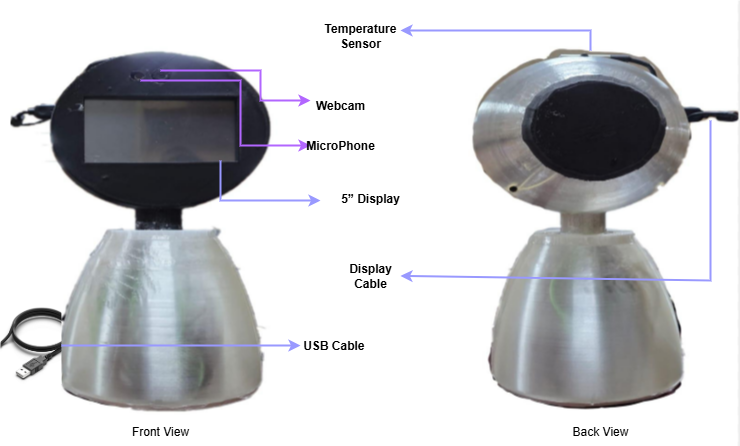
\includegraphics[width=0.6\textwidth]{Medora_thesis (1)/pics/thesis/medora.png}
    \caption{Developed prototype of Medora}
    \label{fig:real-prototype-medora}
\end{figure}

Through this progression from conceptual philosophy to virtual modeling and finally to a working prototype, Medora successfully embodies a design that balances technological sophistication with user-centered accessibility, making it well-suited for daily use in elderly care.


\section{Hardware Implementation}
\subsection{Component Assembly}

The Medora system is a compact, AI-enabled healthcare assistant built around the energy-efficient Raspberry Pi 4B (4GB RAM). It integrates facial and voice recognition,emotion detection, temperature measurement, interaction and voice medicine reminders into one seamless platform.

Upon powering the device with a 5V, 3A USB-C adapter, the Raspberry Pi initializes all connected hardware and software services. A Pi Camera Module (or USB webcam) captures real-time video, enabling AI-driven facial recognition for secure authentication, ensuring that only authorized users can access medications.

For interaction, a USB microphone processes voice commands, allowing natural, hands-free communication. These inputs are handled either locally or via cloud-based NLP services, supporting tasks such as scheduling reminders, requesting medication updates, or checking health information.

To support temperature monitoring, a DS18B20 digital temperature sensor is included to track the user’s body temperature, while a 3.5mm AUX speaker delivers reminders and alerts. An optional 5” HDMI touchscreen is also integrated for enhanced interactivity, providing visual feedback .

Each component was individually tested before full system integration, ensuring compatibility, stability, and reliability. The result is a low-cost, intelligent health assistant capable of secure medication dispensing, continuous health monitoring, and user-friendly interaction—making it especially valuable for elderly care and home-based health management.

\begin{figure}[H]
    \centering
    \includegraphics[width=0.5\textwidth]{Medora_thesis (1)/pics/SSS.png}

    \caption{Hardware Setup}
    \label{fig:Hardware Setup}
\end{figure}

\subsection{Connectivity and Wiring}
\subsection*{1. Raspberry Pi 4 Power}

\begin{itemize}
    \item \textbf{Connection:} \\
    5V 3A USB-C Adapter $\rightarrow$ USB-C Power Port

    \item \textbf{Explanation:} \\
    The Raspberry Pi 4 requires a reliable \textbf{5V, 3A power supply} to operate correctly, especially when using peripherals like cameras or displays. This is delivered through the \textbf{USB-C Power Port}, which is specifically designed to handle the power needs of Pi 4.
\end{itemize}

\subsection*{2. USB Webcam}
\begin{itemize}
 \item \textbf{Connection:} \\
  Webcam USB Cable → Blue USB 3.0 Port

  \item \textbf{Explanation:} \\
 The Raspberry Pi 4 features \textbf{USB 3.0 ports (blue)} which offer faster data transfer speeds. For high-bandwidth devices like webcams, using the USB 3.0 port ensures smoother video capture and better performance. Plugging the webcam into this port enables the Pi to receive the video stream effectively.

 \end{itemize}

\subsection*{3. DS18B20 Temperature Sensor (3-Pin)}

\begin{itemize}
    \item \textbf{Connection Details:}
    \begin{itemize}
        \item VCC (\textit{Left Pin}) $\rightarrow$ 3.3V (Pin 1) – Red wire
        \item GND (\textit{Right Pin}) $\rightarrow$ GND (Pin 6) – Black wire
        \item DATA (\textit{Middle Pin}) $\rightarrow$ GPIO4 (Pin 7) – Yellow wire
        \item 4.7k$\Omega$ Resistor between DATA and VCC (Pin 1)
    \end{itemize}

    \item \textbf{Explanation:} \\
    The \textbf{DS18B20} is a digital temperature sensor that communicates via the \textbf{1-Wire protocol}, typically using \textbf{GPIO4 (Pin 7)} on the Raspberry Pi.
    
    \begin{itemize}
        \item \textbf{VCC} supplies 3.3V power.
        \item \textbf{GND} is the ground reference.
        \item \textbf{DATA} carries the temperature signal and needs to be pulled up to VCC using a \textbf{4.7k$\Omega$ resistor}, ensuring reliable communication.
    \end{itemize}
\end{itemize}

\subsection*{4. AUX Speakerc}
\begin{itemize}
 \item \textbf{Connection:} \\
  3.5mm AUX Jack → Audio Port (3.5mm side port)

  \item \textbf{Explanation:} \\
To output audio, the Raspberry Pi 4 has a \textbf{combined audio/video 3.5mm jack}. By plugging in an \textbf{AUX speaker}, you can hear audio output such as alerts, music, or spoken messages generated by the Pi. No extra configuration is needed if the audio output is set to the headphone jack in the settings.
 
 \end{itemize}

\subsection*{5. 5-inch HDMI Display}

\textbf{Connection:}
\begin{itemize}
    \item \textbf{HDMI Cable} $\rightarrow$ Micro-HDMI Port 0 (closest to USB-C)
    \item \textbf{Optional Power Wires:}
    \begin{itemize}
        \item \textcolor{red}{Red (5V)} $\rightarrow$ Pin 2 or Pin 4 (5V)
        \item \textcolor{black}{Black (GND)} $\rightarrow$ Pin 6 (GND)
    \end{itemize}
\end{itemize}

\textbf{Explanation:}
\begin{itemize}
    \item The Raspberry Pi 4 has \textbf{two Micro-HDMI ports}, with \textbf{Port 0} (closest to the USB-C power) being the \textit{default display output}.
    
    \item A \textbf{5-inch HDMI display} connects via HDMI for video, and may require \textbf{external 5V power}, which can be drawn from the GPIO header (Pins 2 or 4 for 5V, and Pin 6 for GND).
    
    \item This optional power wiring is often needed if the display does not have its own power adapter.
\end{itemize}

This setup enables your Raspberry Pi 4 to operate with stable power while supporting various peripherals for multimedia and sensor integration. It can capture video through a connected webcam, read temperatures using a digital sensor such as the DHT22 or MLX90614, and play sound via USB or 3.5mm jack-connected speakers, including amplified speaker setups. Additionally, it can display a graphical user interface (GUI) or video output on an external HDMI display, making it suitable for a wide range of interactive and real-time applications.

\begin{figure}[H]
    \centering
    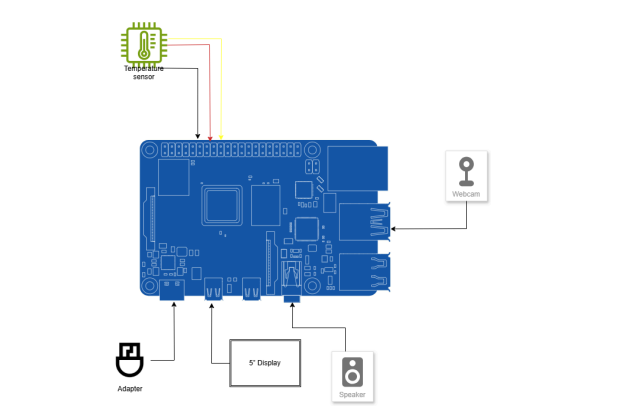
\includegraphics[width=0.8\textwidth]{pics/thesis/circuitdiagram.png}
    \caption{Circuit connection}
    \label{fig: Circuit connection}
\end{figure}



\subsection{ Enclosure and Sensor Mounting}

The external shell of Medora was designed using \textbf{PET-G} material and fabricated via \textbf{3D printing}, incorporating ergonomic considerations for user comfort and functionality. Key features of the enclosure include:

\begin{itemize}
    \item A \textbf{front-mounted USB webcam}, positioned at approximately head height when Medora is placed on a table, to facilitate accurate facial recognition.
    \item An integrated \textbf{speaker port} located behind the facial panel, enabling clear voice output for interactions.
    \item A \textbf{dedicated temperature sensor slot} positioned near the front of the enclosure to effectively capture the user's body heat without requiring physical contact.
    \item \textbf{Ventilation gaps} strategically placed to ensure adequate airflow and maintain thermal safety for the internal Raspberry Pi and other components.
    \item \textbf{Secure compartments} inside the casing to neatly hold the Raspberry Pi, wiring, and breakout boards, minimizing movement and potential damage.
\end{itemize}




\section{Software Deployment and Functional Integration}
Medora integrates multiple software modules to enable real-time perception, 
interaction, and assistance for elderly users. These modules include face detection 
and recognition, emotion detection, temperature sensing, voice-based chatbot, 
text-to-speech (TTS), and reminders. Together, they create a seamless, 
context-aware interaction cycle.

\subsection{Environment Setup and Libraries}

The software for the system was developed in \textbf{Python 3.11} and deployed on 
\textbf{Raspberry Pi OS}. To ensure stability and compatibility, the environment 
was configured as follows:

\begin{itemize}
    \item \textbf{System Update and Upgrade} \\
    The Raspberry Pi was first updated to the latest packages using the \texttt{apt} 
    package manager:
    \begin{verbatim}
    sudo apt update && sudo apt upgrade
    \end{verbatim}

    \item \textbf{Virtual Environment Creation} \\
    A dedicated Python virtual environment was set up to isolate project dependencies 
    and prevent conflicts with system packages:
    \begin{verbatim}
    python3 -m venv medora_env
    source medora_env/bin/activate
    \end{verbatim}

    \item \textbf{Library Installation} \\
    All required Python libraries were installed inside the virtual environment:
    \begin{itemize}
        \item \texttt{face\_recognition} -- for face detection and recognition
        \item \texttt{DeepFace} -- for emotion analysis
        \item \texttt{opencv-python} -- for video capture and image processing
        \item \texttt{pyttsx3} -- for text-to-speech functionality
        \item \texttt{speech\_recognition} -- for voice command processing
        \item \texttt{RPi.GPIO}, \texttt{w1thermsensor} -- for hardware integration and temperature sensing
    \end{itemize}

    \item \textbf{Hardware Configuration} \\
    The Raspberry Pi’s GPIO interfaces and 1-Wire protocol were enabled using the configuration tool:
    \begin{verbatim}
    sudo raspi-config
    \end{verbatim}
\end{itemize}


\subsection*{Integration Stages}

\begin{itemize}
    \item \textbf{Low-Level Integration:}  
    Ensures that sensors, cameras, and microphones deliver correct and reliable input signals.  

    \item \textbf{Mid-Level Integration:}  
    Combines face recognition and emotion detection to provide contextual information 
    about the user.  

    \item \textbf{High-Level Integration:}  
    Links recognition outputs with chatbot, text-to-speech (TTS), and reminder modules. 
    The detected identity and emotional state serve as metadata for generating 
    personalized responses.  
\end{itemize}

\section*{Core Implementation Modules}
\subsection*{Face Detection And Recognition}


\textbf{FACE DETECTION}: For \textbf{FACE DETECTION} Python script uses OpenCV’s Haar Cascade classifier to perform real-time face detection through the webcam. It starts by loading a pre-trained face detection model (\texttt{haarcascade\_frontalface\_default.xml}) and then accesses the default webcam. For each frame captured from the webcam, the image is converted to grayscale to improve detection performance. The face detector scans the grayscale frame and returns coordinates of any detected faces. The script then draws blue rectangles around each detected face in the original color frame. This annotated video feed is displayed in a window titled \texttt{"Face Detection"}. The loop runs continuously until the user presses the ESC key (key code 27), at which point the webcam is released and all OpenCV windows are closed, ending the program.

\textbf{FACE RECOGNITION:}  
The implementation leverages the \texttt{face\_recognition} library in combination with OpenCV to enable real-time face identification. A reference image is first loaded and encoded into a unique facial vector. During execution, the system continuously captures frames from the webcam, converts them into the RGB color space, and extracts facial encodings for each detected face. These encodings are then compared against the stored reference encoding. If a match is identified, the text ``User Recognized'' is displayed on the video stream. This ensures reliable identity verification using facial feature vectors in real time.

\subsection*{FACE RECOGNITION USING OpenCV AND \texttt{face\_recognition} LIBRARY}

\begin{verbatim}
import face_recognition
import cv2

# Load reference image and generate facial encoding
known_image = face_recognition.load_image_file(
    "C:/Users/meshk/Downloads/Face.jpg")
known_encoding = face_recognition.face_encodings(known_image)[0]

# Initialize webcam
cap = cv2.VideoCapture(0)

while True:
    ret, frame = cap.read()
    rgb_frame = frame[:, :, ::-1]  # Convert BGR to RGB
    
    # Detect and encode faces from webcam feed
    face_locations = face_recognition.face_locations(rgb_frame)
    face_encodings = face_recognition.face_encodings(
        rgb_frame, face_locations)

    for face_encoding in face_encodings:
        matches = face_recognition.compare_faces(
            [known_encoding], face_encoding)
        if True in matches:
            cv2.putText(frame, "User Recognized", (50,50), 
                        cv2.FONT_HERSHEY_SIMPLEX, 1, (0,255,0), 2)

    # Show output window
    cv2.imshow("Recognition", frame)
    if cv2.waitKey(1) & 0xFF == 27:  # Press 'Esc' to exit
        break

cap.release()
cv2.destroyAllWindows()
\end{verbatim}


\textbf{EMOTION DETECTION:}  
The system uses the \texttt{DeepFace} library with OpenCV to detect emotional states from a video input. Frames are read sequentially, and every fifth frame is analyzed to balance speed and accuracy. The \texttt{DeepFace.analyze} function processes the frame to identify the dominant facial emotion (e.g., happy, sad, angry). If no face is detected, the system outputs ``No face.'' The detected emotion is then overlaid on the video frame, which is displayed in real time. The program continues until the video ends or the user presses the 'q' key, after which resources are released.

\subsection*{EMOTION DETECTION USING \texttt{DeepFace} LIBRARY}

\begin{verbatim}
# Import necessary libraries
from deepface import DeepFace  # For emotion detection
import cv2  # For video handling and display

# Load the video file
cap = cv2.VideoCapture(r"C:\Users\meshk\Downloads\Emotions.mp4")

# Initialize variables
frame_count = 0
emotion = "Analyzing..."  

while True:
    ret, frame = cap.read()
    if not ret:
        break  # Exit when video ends

    frame_count += 1

    # Analyze every 5th frame for efficiency
    if frame_count % 5 == 0:
        try:
            result = DeepFace.analyze(frame, actions=['emotion'], 
                                      enforce_detection=False)
            emotion = result[0]['dominant_emotion']
        except:
            emotion = "No face"

    # Overlay detected emotion
    cv2.putText(frame, f'Emotion: {emotion}', (20, 50),
                cv2.FONT_HERSHEY_SIMPLEX, 1, (0,255,0), 2)

    cv2.imshow('Emotion Detection (Video)', frame)

    if cv2.waitKey(1) & 0xFF == ord('q'):  # Press 'q' to quit
        break

cap.release()
cv2.destroyAllWindows()
\end{verbatim}

\begin{figure}[H]
    \centering
    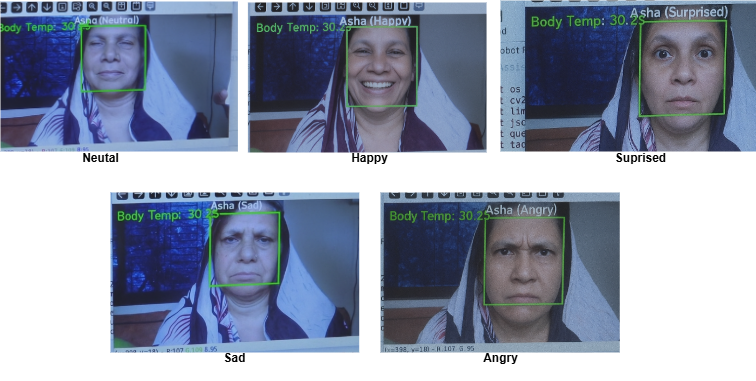
\includegraphics[width=1\textwidth]{Medora_thesis (1)/pics/thesis/ed1.png}
    \caption{Medora detecting emotions from video input using DeepFace}
    \label{fig:medora_emotion_detection}
\end{figure}


\subsection*{Temperature Measurement}
This module measures the user's body temperature using the \texttt{W1ThermSensor} 
library. The sensor communicates with the Raspberry Pi through the 1-Wire protocol 
and provides temperature readings in degrees Celsius.

\begin{verbatim}
from w1thermsensor import W1ThermSensor

# Initialize the sensor
sensor = W1ThermSensor()

# Read temperature
temperature = sensor.get_temperature()

print(f"User temperature: {temperature}°C")
\end{verbatim}

\subsection*{Voice Interaction and Chatbot with TTS}
The voice interaction module enables natural communication with the system. 
It captures user speech via a microphone, converts it into text using the 
\texttt{SpeechRecognition} library, processes the input through a chatbot 
API, and responds with synthesized speech using \texttt{pyttsx3}. This 
enables real-time conversational assistance.

\begin{verbatim}
import speech_recognition as sr
import pyttsx3
import requests

# Initialize text-to-speech engine
engine = pyttsx3.init()

# Initialize recognizer
r = sr.Recognizer()
with sr.Microphone() as source:
    print("Listening...")
    audio = r.listen(source)

try:
    # Convert speech to text
    user_text = r.recognize_google(audio)
except:
    user_text = "Could not understand"

# Send text to chatbot API
API_URL = "https://api.openrouter.ai/v1/chat/completions"
payload = {
    "model": "openai/gpt-3.5-turbo",
    "messages": [{"role": "user", "content": user_text}]
}
response = requests.post(API_URL, json=payload).json()

# Extract chatbot reply
bot_reply = response['choices'][0]['message']['content']

# Speak the response
engine.say(bot_reply)
engine.runAndWait()
\end{verbatim}


\subsection*{Reminder System}

The reminder system enables the robot to deliver time-based notifications, such as 
medication alerts, in a non-intrusive and reliable manner. It is implemented using 
a background process that continuously monitors scheduled reminders.

\begin{itemize}
    \item \textbf{Threaded Implementation} \\
    The system uses Python’s \texttt{threading} module. A separate thread 
    (\texttt{reminder\_loop}) runs concurrently with other modules, ensuring reminders 
    are triggered without interrupting video capture, face recognition, or voice 
    interaction.

    \item \textbf{Task Scheduling} \\
    Each reminder is stored in a list as a dictionary containing the scheduled 
    execution time and the message to be spoken. For example:
    \begin{verbatim}
    {"time": 1692800000, "message": "Take your medicine"}
    \end{verbatim}

    \item \textbf{Continuous Monitoring} \\
    The thread checks the system clock every second. When the scheduled time 
    is reached, the reminder message is delivered through the text-to-speech 
    engine (\texttt{speak()}) and then removed from the task list.

    \item \textbf{Integration with Chatbot} \\
    The GPT-based chatbot enables reminders to be set via natural voice commands. 
    For example:
    \begin{verbatim}
    "Set a reminder in 30s to drink water"
    \end{verbatim}
    is automatically parsed into the internal reminder format.

    \item \textbf{Multithreading Advantage} \\
    Since the reminder system operates in its own thread, the robot can 
    simultaneously perform face recognition, emotion detection, and voice 
    interaction without delay.
\end{itemize}




\subsection{Error Handling and Functional Validation}

To ensure reliability, \textbf{Medora} implements error handling and validation mechanisms as follows:

\begin{itemize}
    \item \textbf{Face \& Emotion Detection:} Missing faces or failed analysis are handled gracefully with default messages.
    \item \textbf{Temperature Sensor:} Sensor errors return default values to avoid misinterpretation.
    \item \textbf{Voice Recognition:} Unclear audio prompts the user to repeat commands.
    \item \textbf{Chatbot/TTS:} API failures are handled with fallback messages.
    \item \textbf{Reminder System:} Conflicts and duplicates are detected and logged.
\end{itemize}

\noindent
\textbf{Functional Validation:}
\begin{itemize}
    \item Modules were tested individually and in integration to ensure real-time responsiveness, accuracy, and minimal latency.
    \item Environmental testing (light, noise, background activity) confirmed system stability.
\end{itemize}


\section{Testing and Calibration }

The Medora is designed to activate and start its functions only after the user says the wake phrase, "Hey Buddy" Once this phrase is detected, the system begins by capturing live video from the camera to perform facial recognition, identifying the user to ensure secure and personalized interaction. Simultaneously, it analyzes the user’s facial expression to detect their current emotional state, which helps tailor the interaction empathetically. The Medora then reads the user's body temperature through the connected sensor, adding a health monitoring layer. After successful recognition and health checks, the system listens for voice commands, allowing the user to naturally request medication reminders, inquire about their temperature, or ask other health-related questions. When the user asks for reminders, the Medora retrieves the scheduled medicines and clearly announces them. Throughout this process, it provides feedback using speech and visual indicators, ensuring a smooth, interactive experience until the session ends or the user issues an exit command.



\begin{figure}[H]
    \centering
    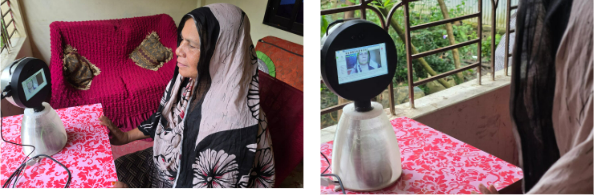
\includegraphics[width=0.7\textwidth]{Medora_thesis (1)/pics/thesis/MI.png}
    \caption{User engaging in interaction with Medora }
    \label{fig: User engaging in interaction with Medora}
\end{figure}


\subsubsection{Sensor Calibration}
The DS18B20 temperature sensor was calibrated against standard thermometers to validate both body and ambient temperature readings. Threshold values for temperature alerts were adjusted according to typical elderly care guidelines. Multiple readings were taken over different sessions to ensure consistency and reliability, resulting in a measurement accuracy within ±0.2°C.

\subsubsection{Camera and Face Recognition Testing}
Face recognition was tested across a variety of conditions including different lighting scenarios, distances, angles, and multiple faces in the camera frame. Each participant’s face was compared against the stored database, and recognition accuracy was calculated as the percentage of correctly identified faces. Adjustments to camera placement and detection parameters ensured robust recognition under normal household conditions,yielding an
overall accuracy of approximately 92\%.

\subsubsection{ Emotion Detection Tuning}
The emotion detection module was tested using both real-time interactions and annotated facial datasets. The system focused on four primary emotions relevant to elderly care: happy, neutral, sad, and angry. Confidence thresholds were tuned to reduce false positives and ensure reliable classification. During testing, subtle expressions such as mild sadness or slight anger were occasionally misclassified, but overall detection accuracy reached
approximately 85\%.

\subsubsection{ Voice and Audio Calibration}
The speech recognition module and text-to-speech (TTS) engine were evaluated for clarity, tone, and responsiveness. Microphone sensitivity was calibrated to capture voice commands reliably within a 2-meter range, while speaker output was tested for clarity in different rooms with moderate background noise. User feedback from elderly participants guided minor adjustments to speech rate and tone to enhance understandability.Overall
voice interaction performance was measured at approximately 88\%.

\subsubsection{ End-to-End Interaction Testing}

The integrated system, encompassing face detection, emotion recognition, chatbot response, TTS output, and reminder alerts, was tested in both controlled laboratory and simulated home environments. Interaction cycles were assessed for latency, coherence, and appropriateness. Response time from face recognition to TTS output was 2-4seconds, and reminders triggered within ±3 seconds of the scheduled time. Errors, delays, and inappropriate responses were logged and addressed iteratively to optimize system performance.

\begin{itemize}
  \item Full system interaction (face detection → emotion recognition → GPT response → speech output) was tested in simulated and real use cases.
  \item Errors, lags, and inappropriate responses were logged and iteratively corrected.
\end{itemize}

These calibration steps ensured that Medora could respond smoothly, accurately, and appropriately during user interaction in daily use settings.

